%------------------------ Packages ------------------------
\documentclass[12pt,a4paper]{article}
\usepackage[latin1]{inputenc}
\usepackage[T1]{fontenc}
\usepackage[pdftex]{graphicx}
\usepackage{float}
\usepackage{amsmath}
\usepackage{amssymb}
\usepackage[FIGTOPCAP]{subfigure}
\usepackage{color}
\usepackage[hidelinks]{hyperref}
\usepackage{listings}
\usepackage[usenames,dvipsnames]{xcolor}
\usepackage[ruled]{algorithm2e}


%-----------------XML----------------
\definecolor{newgrey}{rgb}{0.45,0.25,0.25}
\definecolor{maroon}{rgb}{0.5,0,0}
\definecolor{darkgreen}{rgb}{0,0.5,0}
\lstdefinelanguage{XML}
{
  basicstyle=\footnotesize,
  morestring=[s]{"}{"},
  morecomment=[s]{?}{?},
  morecomment=[s]{!--}{--},
  commentstyle=\color{darkgreen},
  moredelim=[s][\color{black}]{>}{<},
  moredelim=[s][\color{red}]{\ }{=},
  stringstyle=\color{blue},
  identifierstyle=\color{maroon}
}




\lstset{
frame=single,
rulecolor=\color{black!50},
backgroundcolor=\color{gray!7},
}
%-------------------VHDL--------------
\lstdefinelanguage{VHDL}{
  	morekeywords=[1]{
    	library,use,all,entity,is,port,in,out,end,architecture,of,downto,
    	xor,and,nand,or,nor,import,not, signal, variable, process, then, else, elsif,
    	for, while,to, port, map, component, if,begin,and, others         
  	},
	morekeywords=[2]{
     ieee,std,std_logic,std_logic_vector,std_logic_1164,std_logic_arith,std_logic_signed,
     std_logic_unsigned,rising_edge,to_unsigned,to_signed,integer, unsigned, signed
   	},  	
  	morecomment=[l]--,
  	numbers=left,
	numbersep=9pt, % this defines how far the numbers are from the text
}
\colorlet{keyword}{blue!100!black!80}
\colorlet{comment}{green!90!black!90}
\lstdefinestyle{vhdl}{
  language     = VHDL,
  basicstyle   = \scriptsize,
  keywordstyle = [1]\color{keyword}\bfseries,
  keywordstyle = [2]\color{red}\bfseries,
  commentstyle = \color{comment}
}

\newcommand{\version}{\IfFileExists{../../version.txt}
{\input{../../version.txt}}
{\input{../../../version.txt}}
}

\newcommand{\command}[1]{%
\indent \fcolorbox{black}{white}{%
   \begin{minipage}{\dimexpr\textwidth-\parindent\relax}%
      #1
   \end{minipage}%
}
}

\newsavebox{\FVerbBox}
\newenvironment{sample}
{\par \vspace{0.2cm} \begin{lrbox}{\FVerbBox}
\begin{minipage}{\dimexpr\textwidth-\parindent\relax}}
{\end{minipage}
\end{lrbox}
\fcolorbox{black}{lightgray}{\usebox{\FVerbBox}}
\vspace{0.2cm}}

\newenvironment{sampletitle}
{\vspace{0.2cm} \noindent\textbf{Example} :
\begin{sample}}
{\end{sample}}

\newcommand{\samplecomment}[1]{%

\textit{#1}
}

\newcommand{\seealso}[1]{\vspace{0.2cm} \noindent\textbf{See also} :\par #1}

% tikz
\usetikzlibrary{calc}
\usetikzlibrary{arrows}
\usetikzlibrary{shadows}

\tikzset{block/.style={draw, text centered, fill=gray!10,drop shadow}}
\tikzset{connect/.style={draw, line width=1 pt}}

\begin{document}

\tableofcontents

\newpage

\section{Send an image to the smartcam from the computer}

Sometimes, it may be interesting to send an image from the computer to the smart camera.\\

GPStudio provides this opportunity thanks to a simple option.\\

\vspace{0.5cm}

\begin{center}
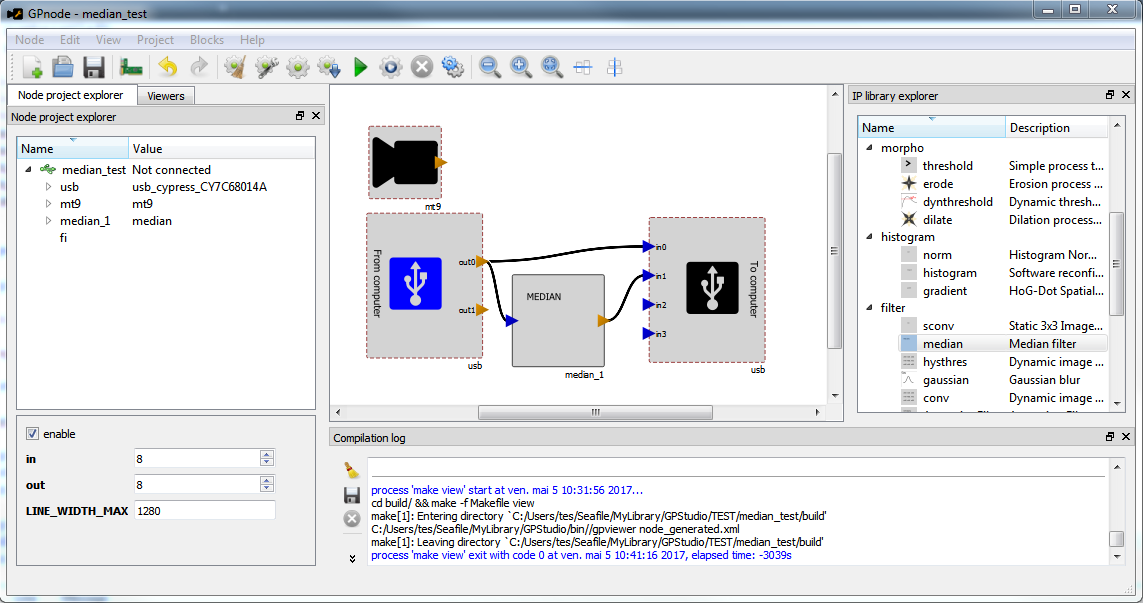
\includegraphics[width=\textwidth]{FC1.png}
\end{center}

\vspace{1cm}

\begin{itemize}
\item First of all, create your project in GPnode as showed on the previous figure and save it.\\ 
\item Generate, compile, send and run the project. \\ 
\item After having generate, compile, send and run the project, you are directed to the GPviewer. In the GPviewer, select "Flow sender".\\ 
\item Select the path to the images that have to be sent to the smart camera.\\
\item Choose the image and send it to the out0 port or the out1 port.  
\end{itemize}

\newpage

The following figure shows the result. \\ 

\begin{center}
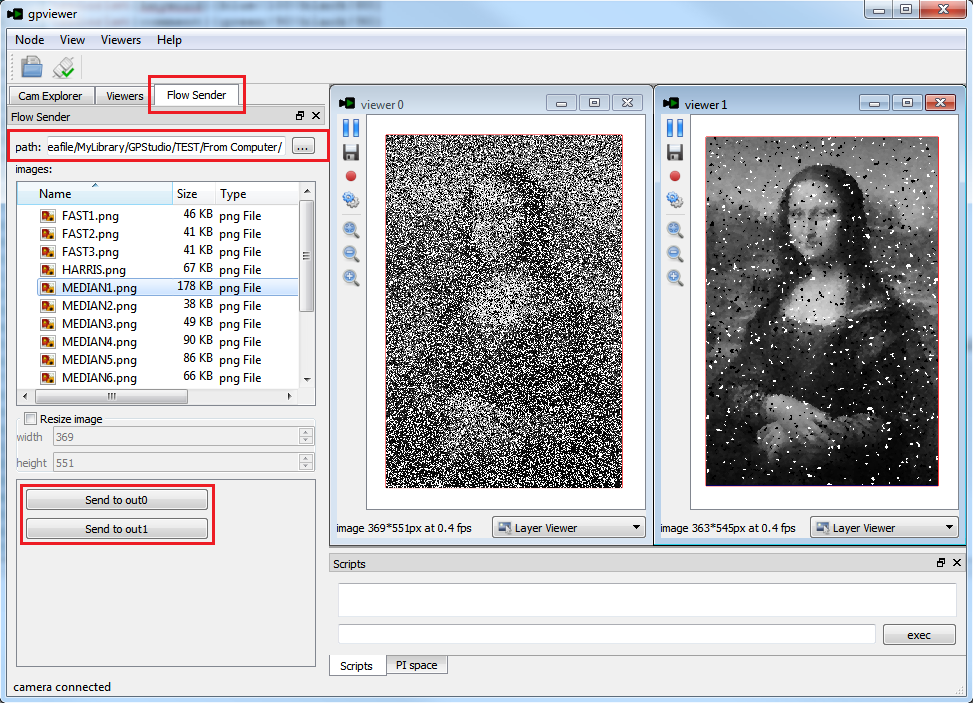
\includegraphics[width=\textwidth]{FC2.png}
\end{center}

\newpage

\section{Draw a rectangle or several points with gpviewer}

\subsection{Rectangle}

\vspace{1.5cm}

\begin{figure}[h!]
\centering
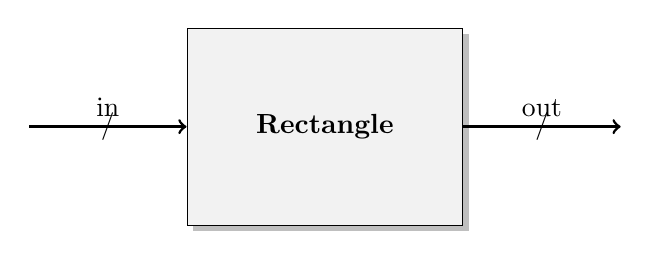
\begin{tikzpicture}
\node[block,rectangle,minimum height=2.5cm,minimum width=3.5cm] (bloc) {\textbf{Rectangle}};

\path[connect,<-] ([yshift=0.0cm]bloc.west) -- node{/} node[above]{in} ++(-2cm,0);

\path[connect,->] ([yshift=0.0cm]bloc.east) -- node{/} node[above]{out} ++(2cm,0);
 ([xshift=0.5cm,yshift=-0.6cm]bloc.north);

\end{tikzpicture}
\end{figure}

\vspace{1cm}

The input flow contains the pixels from the sensor coded on 1 byte. The output flow contains the rectangle coordinates.\\

The rectangle coordinates are sent on a serial format via a 64 bits frame, with the following disposition :

\begin{center}
$< x; y;w; h >$\\
\end{center}

Each component is 16 bits wide and the sending order is left to right, Less Significant Byte first.\\

\vspace{1.5cm}

\underline{To parameter the ip ;}

\vspace{0.2cm}

\begin{itemize}
\item You have to write the follow script in the \textbf{.proc file} for the output flow.\\

\lstset{language=XML}
\begin{lstlisting}
<flow name="coord" size="8" type="out">
    <properties>
    	<property name="datatype" type="flowtype" value="features"/>
        <property name="featuretype" type="featuretype" value="rect"/>
    </properties>
</flow>
\end{lstlisting}

\vspace{2.25cm}

\item To implement the \textbf{\_process.vhd}, read the following script.\\ 

\begin{lstlisting}[style=vhdl]
library IEEE;
use IEEE.STD_LOGIC_1164.all;
use IEEE.NUMERIC_STD.all;
library std;

entity draw_process is
	generic (
	    CLK_PROC_FREQ : integer;
	    IMG_SIZE      : integer;
	    COORD_SIZE    : integer
	);
	port (
	    clk_proc      : in std_logic;
	    reset_n       : in std_logic;
	    
	    ---------------- dynamic parameters ports ---------------
	    status_reg_enable_bit     : in std_logic;
	    inImg_size_reg_in_w_reg   : in std_logic_vector(11 downto 0);
	    inImg_size_reg_in_h_reg   : in std_logic_vector(11 downto 0);
	    
	    ------------------------ Img flow -----------------------
	    Img_data                  : in std_logic_vector(IMG_SIZE-1 downto 0);
	    Img_fv                    : in std_logic;
	    Img_dv                    : in std_logic;
	    
	    ----------------------- coord flow ----------------------
	    coord_data                : out std_logic_vector(COORD_SIZE-1 downto 0);
	    coord_fv                  : out std_logic;
	    coord_dv                  : out std_logic
	);
end draw_process;

architecture rtl of draw_process is

--process data_process vars
signal enabled  : std_logic;

--Coord over serial line related vars
signal frame_buffer                 : std_logic_vector(63 downto 0);
signal frame_buffer_has_been_filled : std_logic;
signal frame_buffer_has_been_sent   : std_logic;
signal frame_buffer_position        : unsigned(6 downto 0);

begin
    data_process : process (clk_proc, reset_n)
    
    begin
         if(reset_n='0') then
            --Cleaning frame buffer
            frame_buffer    <= (others=>'0');
            --Cleaning signals used to fill buffer
            frame_buffer_has_been_filled <= '0';
            frame_buffer_has_been_sent	 <= '0';
            coord_fv 	<= '0';
            coord_dv 	<= '0';
            coord_data 	<= (others=>'0');
            --Cleaning flags
            enabled 	<= '0';

		 elsif(rising_edge(clk_proc)) then
		    coord_fv  	<= '0';
		    coord_dv 	<= '0';
		    coord_data 	<= (others=>'0');
		    
		    if(Img_fv = '0') then
		        --
		        if(frame_buffer_has_been_filled = '0')then
		            --We send frame coordinates only if there is something to send
		            if(enabled = '1' and frame_buffer_has_been_sent = '0')then
		                frame_buffer <= (others => '0');
		                
		                --filling buffer with matching coordinates
		                frame_buffer(15 downto 0)  <= std_logic_vector(to_unsigned(10,16)); -- x
		                frame_buffer(31 downto 16) <= std_logic_vector(to_unsigned(10,16)); -- y
		                frame_buffer(47 downto 32) <= std_logic_vector(to_unsigned(100,16)); -- w
		                frame_buffer(63 downto 48) <= std_logic_vector(to_unsigned(100,16)); -- h
		                
		                -- Get buffer ready to send
		                frame_buffer_has_been_filled <= '1';
		                frame_buffer_position        <= (others=>'0');		                
		            end if;
		        else
		            --send coord
		            coord_fv <= '1';
		            coord_dv <= '1';
		            coord_data <= frame_buffer(to_integer(frame_buffer_position)+7 downto to_integer(frame_buffer_position));
		            
		            if(frame_buffer_position >= 65)then
		                frame_buffer_has_been_filled <= '0';
		                frame_buffer_has_been_sent   <= '1';
		            else
		                frame_buffer_position <= frame_buffer_position + to_unsigned(8,8);
		            end if;
		        end if;
		        enabled  <= status_reg_enable_bit;
		    else
		        coord_fv 	<= '0';
		        coord_dv 	<= '0';
		        coord_data 	<= (others=>'0');
		        frame_buffer_has_been_sent	 <= '0';
		    end if;
		end if;
    end process;
end rtl;
\end{lstlisting}

\newpage



\newpage


\item The last manipulation to do before running the compilation is to add the output flow containning the coordinates in the viewer that receives the output flow from the sensor. As showed at the follow figure.\\ 

\end{itemize}
  

\begin{center}
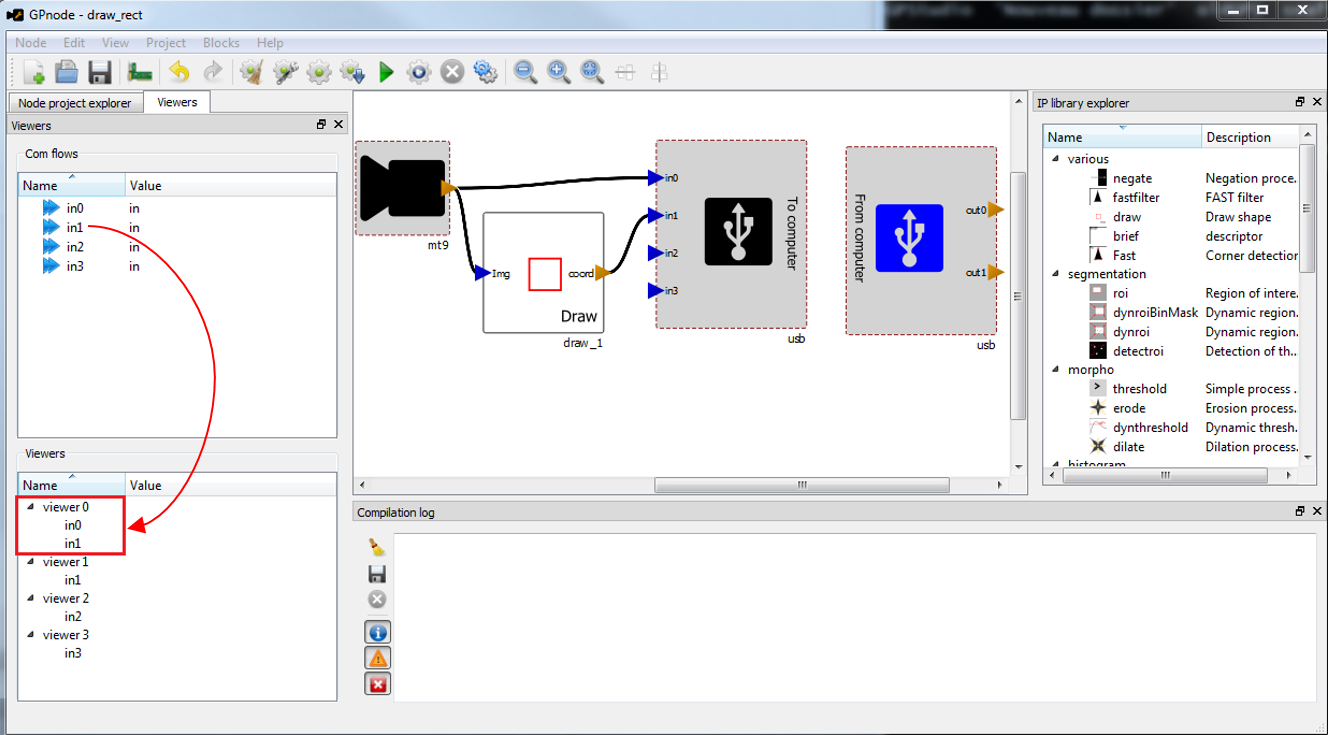
\includegraphics[width=\textwidth]{rect1.png}
\end{center}

\vspace{1cm}

After having run the compilation, we get the follow result in gpviewer.\\
 
\begin{center}
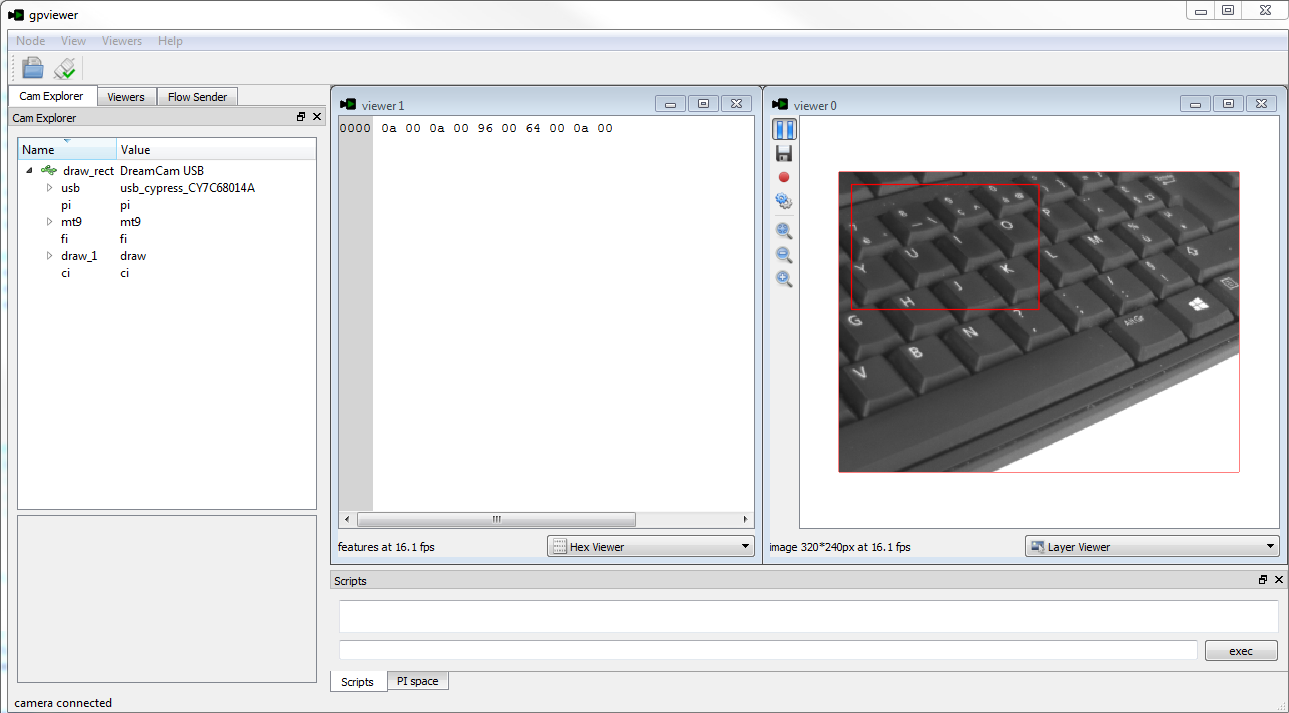
\includegraphics[width=\textwidth]{rect2.png}
\end{center}

\newpage

\subsection{Several points}

\vspace{1.5cm}

\begin{figure}[h!]
\centering
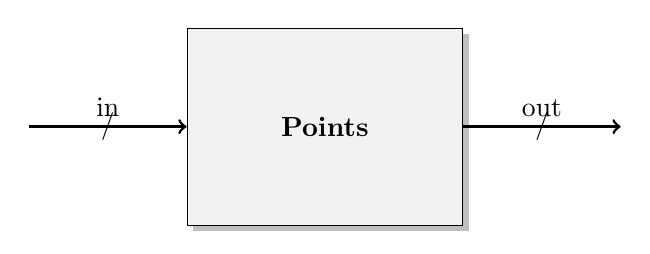
\begin{tikzpicture}
\node[block,rectangle,minimum height=2.5cm,minimum width=3.5cm] (bloc) {\textbf{Points}};

\path[connect,<-] ([yshift=0.0cm]bloc.west) -- node{/} node[above]{in} ++(-2cm,0);

\path[connect,->] ([yshift=0.0cm]bloc.east) -- node{/} node[above]{out} ++(2cm,0);
 ([xshift=0.5cm,yshift=-0.6cm]bloc.north);

\end{tikzpicture}
\end{figure}

To draw several points in a viewer of gpviewer, just modify the value of the featuretype.\\

\lstset{language=XML}
\begin{lstlisting}
<flow name="coord" size="8" type="out">
    <properties>
    	<property name="datatype" type="flowtype" value="features"/>
        <property name="featuretype" type="featuretype" value="point"/>
    </properties>
</flow>
\end{lstlisting}

\vspace{0.5cm}

After having run the compilation, we get the follow result in gpviewer.\\
 
\begin{center}
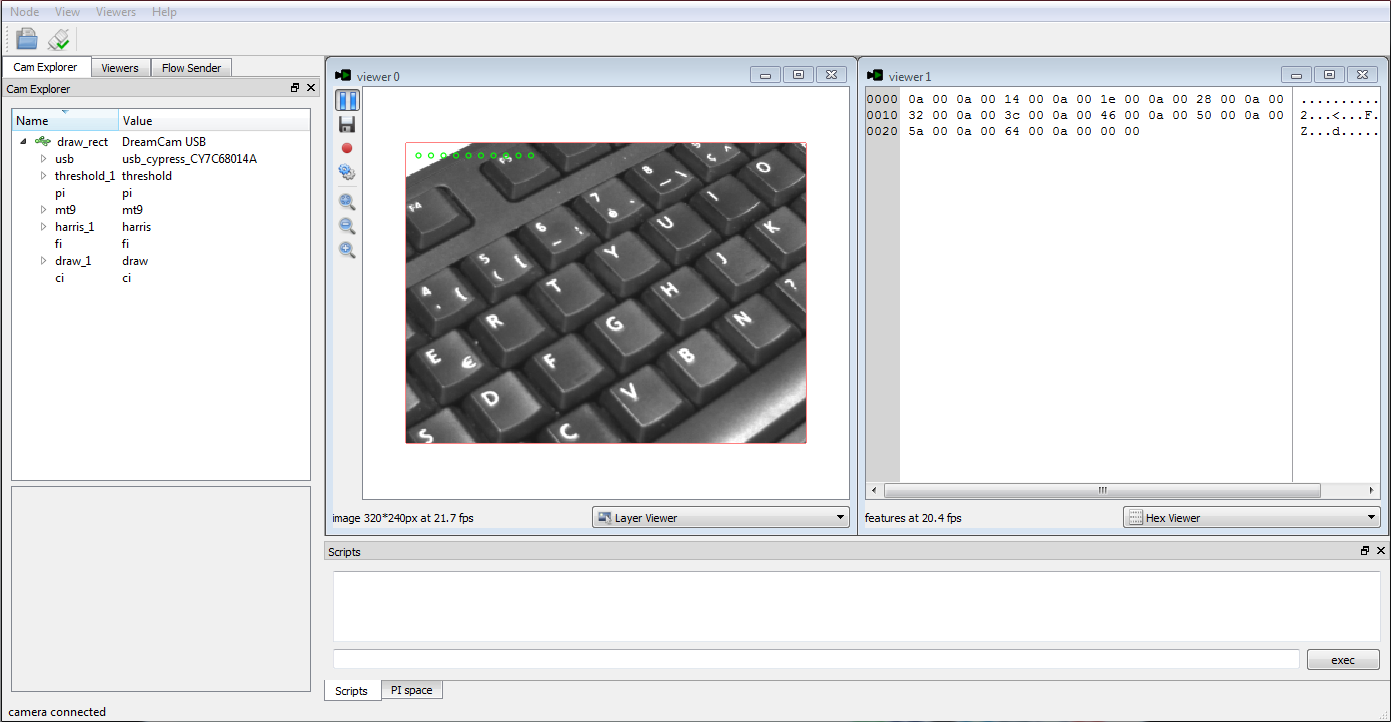
\includegraphics[width=\textwidth]{points.png}
\end{center}

\vspace{0.5cm}

For the both options, draw a rectangle or several points, the main structure of the file is the same. Let see the follow pseudo-code.\\

\begin{algorithm}[H]
 %\KwData{~ $M$\\}
 \vspace{0.1cm}
 \textbf{Initialization}: ~\\\vspace{0.2cm}
 {\footnotesize 
 signal frame\_buffer \\
 signal frame\_buffer\_filled \\
 signal frame\_buffer\_sent \\
 signal frame\_buffer\_position \\
 \vspace{0.2cm}

 	\uIf{(reset = $0$)}
 	{
    \vspace{0.2cm}
   	frame\_buffer $\leftarrow '0...0'$\;
 	frame\_buffer\_filled $\leftarrow '0'$\;
 	frame\_buffer\_sent $\leftarrow '0'$\;
 	\vspace{0.2cm}
  	}
  	\ElseIf{(rising\_edge(clk))}
	{
	\vspace{0.2cm}
	out\_fv $\leftarrow '0'$\;	
	out\_dv $\leftarrow '0'$\; 	
	out\_data $\leftarrow '0...0'$\;
	\vspace{0.2cm}
		\uIf{(in\_fv = $1$)}
 		{
 		\vspace{0.2cm}
		\textcolor{darkgreen}{$\setminus\setminus$ your script}
		\vspace{0.2cm}
  		}
  		\uElseIf{(in\_fv = $0$)}
		{
		\vspace{0.2cm}
			\eIf{(frame\_buffer\_filled = $0$)}
			{
			\vspace{0.2cm}
			\If{(frame\_buffer\_sent = 0)}
			{
			\vspace{0.2cm}
			\textcolor{newgrey}{Filling of the frame buffer\;} \vspace{0.05cm}
			frame\_buffer\_filled $\leftarrow '1'$\;
			frame\_buffer\_position $\leftarrow '0...0'$\;
			\vspace{0.2cm}
			}			
			
			}
			{
			\vspace{0.2cm}
			out\_fv $\leftarrow '1'$\;	
			out\_dv $\leftarrow '1'$\; 	
			out\_data $\leftarrow$ frame\_buffer((frame\_buffer\_position)\\
			\qquad \qquad \qquad + 7 downto (frame\_buffer\_position))\;
			\vspace{0.2cm}

			\eIf{(frame\_buffer\_position $\geq$ $Value\footnote{$Value = 32n+1$, where $n$ is the number of points that you want to send on the output flow. If you want to draw a rectangle, $n = 2$.}$)}
			{
			\vspace{0.2cm}
   			signal frame\_buffer\_sent $\leftarrow '1'$\;
 			signal frame\_buffer\_filled $\leftarrow '0'$\;
 			\vspace{0.2cm}
			}
			{
			\vspace{0.2cm}
			\textcolor{newgrey}{Incrementation of the frame\_buffer\_position value\;}
			\vspace{0.2cm}
			}	
			}		
		}
		\Else
		{
		\vspace{0.2cm}
		out\_fv $\leftarrow '0'$\;	
		out\_dv $\leftarrow '0'$\; 	
		out\_data $\leftarrow '0...0'$\;
		frame\_buffer\_sent $\leftarrow '0'$\;
		\vspace{0.2cm}
		} 	 	
	} 
 }
 
 %\caption{ }
\end{algorithm}


\end{document}